\chapter{Introduzione}
\section{Rappresentazione di numeri reali rispetto ad una base}
\begin{esempio}
    Cosa vuol dire scrivere $12.211$ rispetto ad una certa base?

    Sia dato il numero $12.211$ in base $10$. Questo numero può essere scritto
    come:
    \begin{equation*}
        12.211_{10} = 1\cdot 10^1+2\cdot 10^0 +2 \cdot 10^{-1} + 1 \cdot 10^{-2}
        + 1 \cdot 10^{-3}
    \end{equation*}
    Oppure, utilizzando una base diversa possiamo scrivere:
    \begin{equation*}
        12.211_{3} = 1\cdot 3^1+2\cdot 3^0 +2 \cdot 3^{-1} + 1 \cdot 3^{-2}
        + 1 \cdot 3^{-3}
    \end{equation*}
\end{esempio}
\begin{definizione}[\textbf{Rappresentazione rispetto ad una base}]
    Sia $\beta$ una base. Un numero $x$ è rappresentato in base $\beta$ come:
    \begin{equation}
        \pm a_n a_{n-1} \dots a_{-m} = \pm \sum_{j = -m}^{n} a_j \cdot \beta^j
    \end{equation}
    con $a_j \in \{0, 1, \dots, \beta-1\}$ e $a_n \neq 0$.
\end{definizione}
\begin{teorema}
    $1=0.\overline{9}$
    \begin{proof}
        Possiamo dire che:
        \begin{equation*}
            0.\overline{9} = \sum_{j = 1}^{+ \infty} 9 \cdot 10^{-j} = 9
            \sum_{j=0}^{+\infty} \cdot 10^{-j-1} = 9 \sum_{j = 0}^{+\infty} \cdot
            \frac{1}{10}^{j+1} = \frac{9}{10} \sum _{j=0}^{+\infty} \cdot \frac{1}{10}^{j} =
            = \frac{9}{10} \cdot \frac{1}{1-\frac{1}{10}} = 1
        \end{equation*}
    \end{proof}
\end{teorema}
\begin{teorema}
    Sia dato $\frac{p}{q}$ un numero razionale ai minimi termini. Tale numero ha
    una rappresentazione \textbf{finita} se e solo se tutti divisori primi di $q$
    dividono anche la base $\beta$.
\end{teorema}
Questo teorema ci permette di affermare che sui computer non possiamo
rappresentare i numeri reali e razionali perfettamente. Questo è dovuto al fatto
che la base utilizzata dai computer è la base $2$ e quindi il denominatore deve
essere divisibile per $2$ per avere una rappresentazione finita.
\section{Aritmetica floating point}
\begin{definizione}[\textbf{Aritemtica}]
    Sia $F$ un insieme di numeri rappresentabile su un computer. Un'aritmetica
    di macchina per $F$ è una quadrupla:
    \begin{equation}
        (\beta, t, L, U)
    \end{equation}
    dove:
    \begin{itemize}
        \item $\beta$: è la base
        \item $t$: è la \textbf{mantissa}, quanti numeri posso mettere prima e
              dopo la virgola
        \item $L$: lower bound ($< 0$)
        \item $U$: upper bound ($> 0$)
    \end{itemize}
\end{definizione}
$F$ consiste dei numeri rappresentabili attraverso la seguente formula:
\begin{equation}
    \pm 0.a_1a_2\dots a_t\cdot \beta ^e
\end{equation}
con $a_1 \neq 0$, $0 \leq a_j \leq \beta-1$, $L\leq e \leq U$.
\subsection{Standard Double Precision}
Analizziamo ora lo \textbf{Standard Double Precision} nel quale la quadrupla è
definita come:
\begin{equation}
    (\beta = 2, t = 52 + 1, L = -1022, U = 1023)
\end{equation}
La mantissa è composta da $53$ bit, ma il primo bit è sempre $1$ quindi non lo
si considera, il che ci lascia con una mantissa composta da $52$ bit. In aggiunta
per l'esponente può assumere $2^{11} - 2 = 2046$ valori, ovvero possiamo rappresentare
l'esponente utilizzando $11$ bit.

Solitamente sui computer viene utilizzato un sistema a $64$ bit di cui:
\begin{itemize}
    \item $1$ bit: per rappresentare il segno.
    \item $11$ bit: per l'esponente. Nella realtà si utilizzano 2046 valori per
          rappresentare l'esponente, il che corrisponde a $2^{11} - 2$. Le due
          configurazioni aggiuntive servono per rappresentare \texttt{Inf} e
          \texttt{NaN}.
    \item $52$ bit: per rappresentare la mantissa.
\end{itemize}
\begin{figure}[!ht]
    \centering
    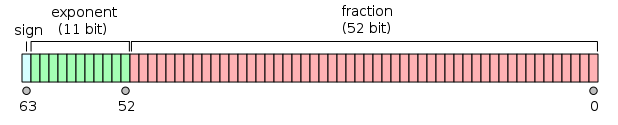
\includegraphics[width=0.7\textwidth]{./img/intro/floatnumber.png}
    \caption{Rappresentazione di un numero in aritmetica floating point}
\end{figure}
\subsection{Operazioni in Aritmetica floating point}
Vediamo ora come vengono effettuate le operazioni in aritmetica floating point.
Calcolare la somma tra due numeri floating point $x,y$ coincide a col calcolare:
\begin{equation}
    x \oplus y = fl(fl(x) + fl(y))
\end{equation}
Dove $fl(z)$ con $z\in \mathbb{R}$ è la rappresentazione l'approssimazione del
numero $z$ nell'aritmetica floating point.
\begin{nota}
    Alcune funzioni, come ad esempio $\sin(z)$, sono rappresentate utilizzando
    la serie di Taylor.
\end{nota}
\begin{definizione} [\textbf{Errore assoluto}]
    Se $x$ è una quantità \textbf{esatta}, sia $\stackrel{\sim}{x}$ la quantità
    approssimata relativa, sia $\|\cdot\|$ una misura di errore, allora
    l'\textbf{errore assoluto} si ottiene come:
    \begin{equation}
        \|x-\stackrel{\sim}{x}\|
    \end{equation}
\end{definizione}
\begin{definizione} [\textbf{Errore relativo}]
    Se $x$ è una quantità \textbf{esatta}, sia $\stackrel{\sim}{x}$ la quantità
    approssimata relativa, sia $\|\cdot\|$ una misura di errore, allora
    l'\textbf{errore relativo} si ottiene come:
    \begin{equation}
        \frac{\|x-\stackrel{\sim}{x}\|}{\|x\|}
    \end{equation}
\end{definizione}
Avendo definito la misura di errore, possiamo calcolare:
\begin{equation}
    \frac{\|(x+y)-(x\oplus y)\|}{\|x+y\|}
\end{equation}
Questa misura di errore può essere semplifica ottenendo il seguente risultato:
\begin{equation}
    \begin{aligned}
        \frac{|x + y - fl(x) + fl(y)|}{|x + y|} = \frac{\|(x + y) - (x (1 +
        \varepsilon_x) + y(1 + \varepsilon_y)) \cdot (1 + \varepsilon_+)\|}{\|x + y\|} = \\
        \frac{|x \varepsilon_x + y \varepsilon_y + (x + y) \varepsilon_S + x
            \varepsilon_x \varepsilon_S + Y \varepsilon_y \varepsilon_S|}{|x + y|} =
        \approx \frac{\left|\frac{x}{x + y} \varepsilon_x + \frac{y}{x + y}
            \varepsilon_y \varepsilon_S \right|}{|x + y|} \leq \left|\frac{x}{x + y}
        \right| \varepsilon_x + \left|\frac{y}{x + y}\right| \varepsilon_y + \varepsilon_S
    \end{aligned}
\end{equation}
Per $\varepsilon$ piccolo l'errore cresce quando $y \sim -x$. Quindi la somma
\textbf{non è stabile} e l'errore aumenta quando $x + y \sim 0$.
\begin{esempio}
    Ad esempio analizzando le seguenti funzioni, le quali sono identiche dal
    punto di vista matematico, si ottengono risultati diversi:
    \begin{equation*}
        f(x) = \sqrt{x + 1} - \sqrt{x}
    \end{equation*}
    \begin{equation*}
        g(x) = \frac{1}{\sqrt{x + 1} + \sqrt{x}}
    \end{equation*}
    Il risultato di $f(x)$ è instabile per grandi valori di $x$, mentre il
    risultato di $g(x)$ è stabile.
\end{esempio}
Per quanto riguarda il \textbf{prodotto} è possibile effettuare lo stesso
ragionamento. In questo caso calcoliamo:
\begin{equation}
    \frac{\|(x\cdot y)-(x\odot y)\|}{\|x\cdot y\|}
\end{equation}
Questa misura di errore può essere semplifica ottenendo il seguente risultato:
\begin{equation}
    \begin{aligned}
        \frac{|x \cdot y - fl(x) \cdot fl(y)|}{|x \cdot y|} = \frac{|xy - xy(1 +
        \varepsilon_x)(1 + \varepsilon_y)(1 + \varepsilon_P)|}{|xy|} = \\
        = |1 - (1 + \varepsilon_x)(1 + \varepsilon_y)(1 + \varepsilon_P)| =
        |\varepsilon_x + \varepsilon_y + \varepsilon_P + \varepsilon_x \varepsilon_y
        + \varepsilon_x \varepsilon_P + \varepsilon_y \varepsilon_P + \varepsilon_x
        \varepsilon_y \varepsilon_P| \approx                           \\
        \approx |\varepsilon_x + \varepsilon_y + \varepsilon_P| \leq 3\varepsilon
    \end{aligned}
\end{equation}
stesse semplificazioni si ottiene che il prodotto è \textbf{stabile} quindi perché
rimangono solo gli $\varepsilon$ che sono tendenti a $0$.